\chapter{الگوریتم‌های حریصانه}

\index{الگوریتم حریصانه}

یک \key{الگوریتم حریصانه}
با انجام انتخابی که در لحظه بهترین به نظر می‌رسد،
راه‌حلی برای مسئله می‌سازد.
الگوریتم حریصانه هرگز از انتخاب‌های خود عقب‌نشینی نمی‌کند،
بلکه مستقیماً راه‌حل نهایی را می‌سازد.
به همین دلیل، الگوریتم‌های حریصانه
معمولاً بسیار کارآمد هستند.

دشواری در طراحی الگوریتم‌های حریصانه،
یافتن راهبردی حریصانه است
که همیشه راه‌حل بهینه مسئله را تولید کند.
انتخاب‌های بهینه محلی در یک الگوریتم حریصانه
باید از نظر سراسری نیز بهینه باشند.
اثبات درستی عملکرد یک الگوریتم حریصانه اغلب دشوار است.

\section{مسئله سکه}

به عنوان نخستین مثال، مسئله‌ای را بررسی می‌کنیم
که در آن مجموعه‌ای از سکه‌ها داده شده است
و هدف، ساختن مبلغ $n$ با استفاده از این سکه‌ها است.
ارزش سکه‌ها برابر با
$\texttt{coins}=\{c_1,c_2,\ldots,c_k\}$
است و از هر سکه می‌توان به تعداد دلخواه استفاده کرد.
حداقل تعداد سکه‌های مورد نیاز چقدر است؟

برای نمونه، اگر سکه‌ها سکه‌های یورو (به سنت) باشند:
\[\{1,2,5,10,20,50,100,200\}\]
و $n=520$ باشد،
حداقل به چهار سکه نیاز داریم.
راه‌حل بهینه، انتخاب سکه‌های
$200+200+100+20$ است که مجموع آن‌ها ۵۲۰ می‌شود.

\subsubsection{الگوریتم حریصانه}

یک الگوریتم حریصانه ساده برای این مسئله،
همواره بزرگ‌ترین سکه ممکن را برمی‌گزیند
تا زمانی که مبلغ مورد نظر ساخته شود.
این الگوریتم در مثال بالا کار می‌کند،
زیرا ابتدا دو سکه ۲۰۰ سنتی،
سپس یک سکه ۱۰۰ سنتی و در پایان یک سکه ۲۰ سنتی انتخاب می‌کنیم.
اما آیا این الگوریتم همواره کار می‌کند؟

مشخص می‌شود که اگر سکه‌ها از نوع یورو باشند،
الگوریتم حریصانه \emph{همیشه} کار می‌کند؛ یعنی
همواره راه‌حلی با کمترین تعداد سکه ممکن به دست می‌دهد.
درستی این الگوریتم را می‌توان به صورت زیر نشان داد:

نخست، هر یک از سکه‌های ۱، ۵، ۱۰، ۵۰ و ۱۰۰
حداکثر یک بار در یک راه‌حل بهینه ظاهر می‌شوند،
زیرا اگر راه‌حل شامل دو عدد از این سکه‌ها باشد،
می‌توان آن‌ها را با یک سکه جایگزین کرد و
راه‌حل بهتری به دست آورد.
برای نمونه، اگر راه‌حل شامل سکه‌های $5+5$ باشد،
می‌توان آن‌ها را با سکه $10$ جایگزین کرد.

به همین ترتیب، سکه‌های ۲ و ۲۰
حداکثر دو بار در یک راه‌حل بهینه ظاهر می‌شوند،
زیرا می‌توان سکه‌های $2+2+2$ را با سکه‌های $5+1$ و
سکه‌های $20+20+20$ را با سکه‌های $50+10$ جایگزین کرد.
علاوه بر این، یک راه‌حل بهینه نمی‌تواند شامل
سکه‌های $2+2+1$ یا $20+20+10$ باشد،
زیرا می‌توان آن‌ها را با سکه‌های $5$ و $50$ جایگزین کرد.

با استفاده از این مشاهدات،
می‌توان برای هر سکه $x$ نشان داد که
ساختن بهینه مجموع $x$ یا هر مبلغ بزرگ‌تر از آن،
تنها با استفاده از سکه‌های کوچک‌تر از $x$ غیرممکن است.
برای نمونه، اگر $x=100$ باشد، بزرگ‌ترین مجموع بهینه
با استفاده از سکه‌های کوچک‌تر برابر است با: $50+20+20+5+2+2=99$.
بنابراین، الگوریتم حریصانه‌ای که همیشه بزرگ‌ترین سکه را انتخاب می‌کند،
راه‌حل بهینه را به دست می‌دهد.

این مثال نشان می‌دهد که اثبات درستی یک الگوریتم حریصانه
می‌تواند دشوار باشد، حتی اگر خود الگوریتم ساده باشد.

\subsubsection{حالت کلی}

در حالت کلی، مجموعه سکه‌ها می‌تواند شامل هر مقداری باشد
و الگوریتم حریصانه \emph{لزوماً} راه‌حل بهینه را تولید نمی‌کند.

می‌توان اثبات کرد که یک الگوریتم حریصانه کار نمی‌کند
با نشان دادن یک مثال نقض
که در آن الگوریتم پاسخ نادرست می‌دهد.
در این مسئله می‌توان به سادگی یک مثال نقض پیدا کرد:
اگر سکه‌ها $\{1,3,4\}$ باشند و مجموع هدف
برابر ۶ باشد، الگوریتم حریصانه پاسخ
$4+1+1$ را تولید می‌کند در حالی که پاسخ بهینه $3+3$ است.

مشخص نیست که آیا مسئله سکه عمومی
با هیچ الگوریتم حریصانه‌ای قابل حل است یا خیر\footnote{با این حال، ممکن است
در زمان چندجمله‌ای \emph{بررسی} کرد
که آیا الگوریتم حریصانه ارائه شده در این فصل برای
مجموعه مشخصی از سکه‌ها کار می‌کند یا خیر \cite{pea05}.}.
اما همان‌طور که در فصل ۷ خواهیم دید،
در برخی موارد،
مسئله عمومی را می‌توان به طور کارآمد
با استفاده از یک الگوریتم برنامه‌نویسی پویا
که همیشه پاسخ درست می‌دهد حل کرد.

\section{زمان‌بندی}

بسیاری از مسائل زمان‌بندی را می‌توان
با استفاده از الگوریتم‌های حریصانه حل کرد.
یک مسئله کلاسیک به شرح زیر است:
با فرض $n$ رویداد همراه با زمان‌های شروع و پایان
آن‌ها، برنامه‌ای پیدا کنید
که شامل بیشترین تعداد رویداد ممکن باشد.
انتخاب بخشی از یک رویداد امکان‌پذیر نیست.
برای مثال، رویدادهای زیر را در نظر بگیرید:
\begin{center}
\begin{tabular}{lll}
رویداد & زمان شروع & زمان پایان \\
\hline
$A$ & 1 & 3 \\
$B$ & 2 & 5 \\
$C$ & 3 & 9 \\
$D$ & 6 & 8 \\
\end{tabular}
\end{center}
در این حالت بیشترین تعداد رویدادها دو است.
برای مثال، می‌توانیم رویدادهای $B$ و $D$ را
به صورت زیر انتخاب کنیم:
\begin{center}
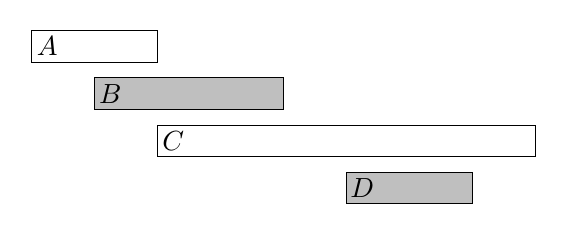
\begin{tikzpicture}[scale=.4]
  \begin{scope}
    \draw (2, 0) rectangle (6, -1);
    \draw[fill=lightgray] (4, -1.5) rectangle (10, -2.5);
    \draw (6, -3) rectangle (18, -4);
    \draw[fill=lightgray] (12, -4.5) rectangle (16, -5.5);
    \node at (2.5,-0.5) {$A$};
    \node at (4.5,-2) {$B$};
    \node at (6.5,-3.5) {$C$};
    \node at (12.5,-5) {$D$};
  \end{scope}
\end{tikzpicture}
\end{center}

می‌توان چندین الگوریتم حریصانه برای
مسئله ابداع کرد، اما کدام‌یک در هر حالتی درست کار می‌کند؟

\subsubsection*{الگوریتم ۱}

ایده اول انتخاب رویدادهایی است که تا حد امکان \emph{کوتاه}
باشند.
در مثال نمونه، این الگوریتم
رویدادهای زیر را انتخاب می‌کند:
\begin{center}
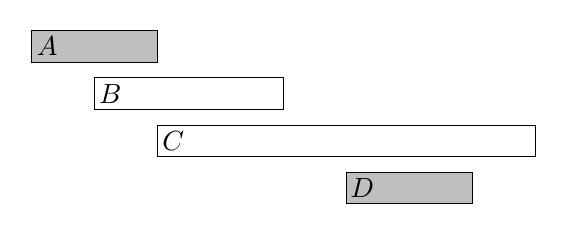
\begin{tikzpicture}[scale=.4]
  \begin{scope}
    \draw[fill=lightgray] (2, 0) rectangle (6, -1);
    \draw (4, -1.5) rectangle (10, -2.5);
    \draw (6, -3) rectangle (18, -4);
    \draw[fill=lightgray] (12, -4.5) rectangle (16, -5.5);
    \node at (2.5,-0.5) {$A$};
    \node at (4.5,-2) {$B$};
    \node at (6.5,-3.5) {$C$};
    \node at (12.5,-5) {$D$};
  \end{scope}
\end{tikzpicture}
\end{center}

اما انتخاب رویدادهای کوتاه همیشه
استراتژی درستی نیست. برای مثال، الگوریتم در
حالت زیر شکست می‌خورد:
\begin{center}
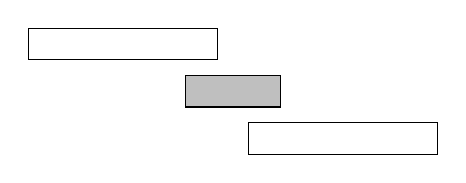
\begin{tikzpicture}[scale=.4]
  \begin{scope}
    \draw (1, 0) rectangle (7, -1);
    \draw[fill=lightgray] (6, -1.5) rectangle (9, -2.5);
    \draw (8, -3) rectangle (14, -4);
  \end{scope}
\end{tikzpicture}
\end{center}
اگر رویداد کوتاه را انتخاب کنیم، فقط می‌توانیم یک رویداد را انتخاب کنیم.
با این حال، امکان انتخاب هر دو رویداد بلند وجود داشت.

\subsubsection*{الگوریتم ۲}

ایدهٔ دیگر این است که همیشه رویداد ممکن بعدی را انتخاب کنیم که تا حد امکان \emph{زودتر} \emph{شروع} می‌شود.
این الگوریتم رویدادهای زیر را انتخاب می‌کند:
\begin{center}
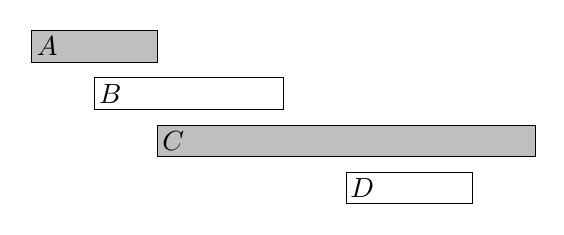
\begin{tikzpicture}[scale=.4]
  \begin{scope}
    \draw[fill=lightgray] (2, 0) rectangle (6, -1);
    \draw (4, -1.5) rectangle (10, -2.5);
    \draw[fill=lightgray] (6, -3) rectangle (18, -4);
    \draw (12, -4.5) rectangle (16, -5.5);
    \node at (2.5,-0.5) {$A$};
    \node at (4.5,-2) {$B$};
    \node at (6.5,-3.5) {$C$};
    \node at (12.5,-5) {$D$};
  \end{scope}
\end{tikzpicture}
\end{center}

با این حال، می‌توانیم برای این الگوریتم نیز یک مثال نقض پیدا کنیم.
به عنوان مثال، در حالت زیر،
الگوریتم فقط یک رویداد را انتخاب می‌کند:
\begin{center}
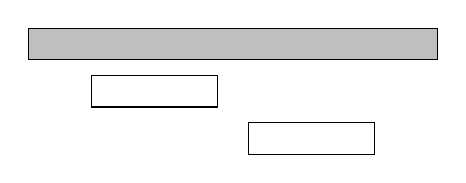
\begin{tikzpicture}[scale=.4]
  \begin{scope}
    \draw[fill=lightgray] (1, 0) rectangle (14, -1);
    \draw (3, -1.5) rectangle (7, -2.5);
    \draw (8, -3) rectangle (12, -4);
  \end{scope}
\end{tikzpicture}
\end{center}
اگر رویداد اول را انتخاب کنیم، انتخاب هیچ رویداد دیگری ممکن نخواهد بود.
در حالی که انتخاب دو رویداد دیگر ممکن بود.

\subsubsection*{الگوریتم ۳}

ایدهٔ سوم این است که همیشه رویداد ممکن بعدی را انتخاب کنیم که تا حد امکان \emph{زودتر} \emph{پایان} می‌یابد.
این الگوریتم رویدادهای زیر را انتخاب می‌کند: 
\begin{center}
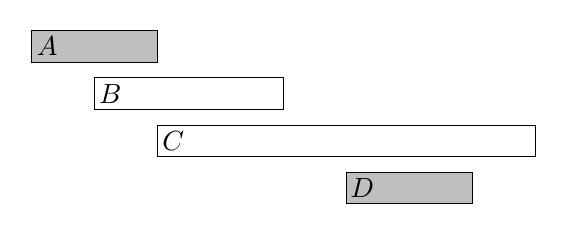
\begin{tikzpicture}[scale=.4]
  \begin{scope}
    \draw[fill=lightgray] (2, 0) rectangle (6, -1);
    \draw (4, -1.5) rectangle (10, -2.5);
    \draw (6, -3) rectangle (18, -4);
    \draw[fill=lightgray] (12, -4.5) rectangle (16, -5.5);
    \node at (2.5,-0.5) {$A$};
    \node at (4.5,-2) {$B$};
    \node at (6.5,-3.5) {$C$};
    \node at (12.5,-5) {$D$};
  \end{scope}
\end{tikzpicture}
\end{center}

مشخص می‌شود که این الگوریتم \emph{همیشه} یک پاسخ بهینه تولید می‌کند.
دلیل این امر آن است که انتخاب رویدادی که در زودترین زمان ممکن پایان می‌یابد، در گام اول همواره یک انتخاب بهینه است.
پس از آن نیز انتخاب رویداد بعدی با استفاده از همین استراتژی انتخابی بهینه خواهد بود، و به همین ترتیب،
تا زمانی که دیگر نتوان رویدادی را انتخاب کرد.

یک روش برای اثبات درستی الگوریتم این است که بررسی کنیم
چه اتفاقی می‌افتد اگر ابتدا رویدادی را انتخاب کنیم
که دیرتر از رویداد با زودترین زمان پایان، تمام می‌شود.
در این وضعیت، برای انتخاب رویداد بعدی حداکثر به همان اندازه (یا کمتر) انتخاب خواهیم داشت.
بنابراین، انتخاب رویدادی که دیرتر تمام می‌شود هرگز نمی‌تواند پاسخ بهتری ایجاد کند،
و الگوریتم حریصانه درست است.

\section{وظایف و مهلت‌ها}

اکنون مسئله‌ای را در نظر بگیرید که در آن
$n$ وظیفه با مدت‌زمان و مهلت معین داده شده‌اند
و هدف ما انتخاب ترتیبی برای انجام این وظایف است.
به ازای هر وظیفه، $d-x$ امتیاز کسب می‌کنیم
که در آن $d$ مهلت انجام وظیفه
و $x$ زمانی است که وظیفه را به پایان می‌رسانیم.
بیشترین مجموع امتیاز ممکن که می‌توانیم به دست آوریم چقدر است؟

برای مثال، فرض کنید کارها به صورت زیر باشند:
\begin{center}
\begin{tabular}{lll}
کار & مدت زمان & مهلت زمانی \\
\hline
$A$ & 4 & 2 \\
$B$ & 3 & 5 \\
$C$ & 2 & 7 \\
$D$ & 4 & 5 \\
\end{tabular}
\end{center}
در این حالت، یک زمان‌بندی بهینه برای کارها به صورت زیر است:
\begin{center}
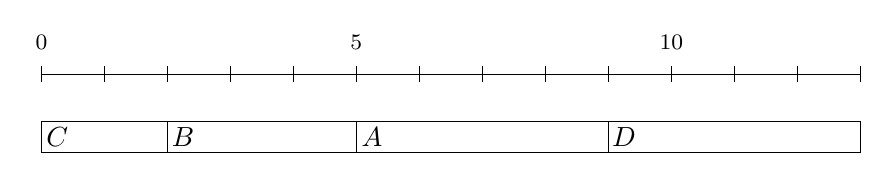
\begin{tikzpicture}[scale=.4]
  \begin{scope}
    \draw (0, 0) rectangle (4, -1);
    \draw (4, 0) rectangle (10, -1);
    \draw (10, 0) rectangle (18, -1);
    \draw (18, 0) rectangle (26, -1);
    \node at (0.5,-0.5) {$C$};
    \node at (4.5,-0.5) {$B$};
    \node at (10.5,-0.5) {$A$};
    \node at (18.5,-0.5) {$D$};

    \draw (0,1.5) -- (26,1.5);
    \foreach \i in {0,2,...,26}
    {
        \draw (\i,1.25) -- (\i,1.75);
    }
    \footnotesize
    \node at (0,2.5) {0};
    \node at (10,2.5) {5};
    \node at (20,2.5) {10};

  \end{scope}
\end{tikzpicture}
\end{center}
در این راه‌حل، $C$ به میزان 5 امتیاز، $B$ به میزان 0 امتیاز، $A$ به میزان $-7$ امتیاز و $D$ به میزان $-8$ امتیاز به همراه دارند، بنابراین مجموع امتیازات $-10$ است.

به‌طور شگفت‌آوری، راه‌حل بهینه این مسئله اصلاً به مهلت‌های زمانی بستگی ندارد؛ یک راهبرد حریصانه صحیح آن است که کارها صرفاً \emph{بر اساس مدت زمان آن‌ها به‌صورت صعودی مرتب‌سازی شوند} و سپس انجام گیرند.
دلیل این موضوع آن است که اگر هر بار دو کار را پشت سر هم انجام دهیم طوری که انجام کار اول طولانی‌تر از کار دوم باشد، با جابه‌جا کردن این دو کار می‌توان به راه‌حل بهتری دست یافت.
برای مثال، زمان‌بندی زیر را در نظر بگیرید:
\begin{center}
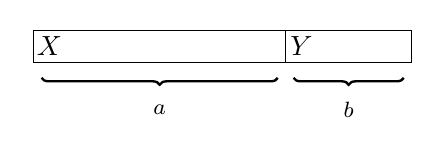
\begin{tikzpicture}[scale=.4]
  \begin{scope}
    \draw (0, 0) rectangle (8, -1);
    \draw (8, 0) rectangle (12, -1);
    \node at (0.5,-0.5) {$X$};
    \node at (8.5,-0.5) {$Y$};

\draw [decoration={brace}, decorate, line width=0.3mm] (7.75,-1.5) -- (0.25,-1.5);
\draw [decoration={brace}, decorate, line width=0.3mm] (11.75,-1.5) -- (8.25,-1.5);

\footnotesize
\node at (4,-2.5) {$a$};
\node at (10,-2.5) {$b$};

  \end{scope}
\end{tikzpicture}
\end{center}
در اینجا $a>b$ است، بنابراین باید کارها را جابه‌جا کنیم:
\begin{center}
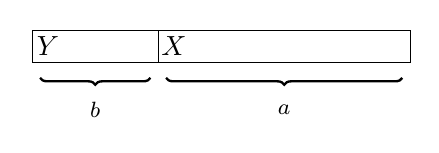
\begin{tikzpicture}[scale=.4]
  \begin{scope}
    \draw (0, 0) rectangle (4, -1);
    \draw (4, 0) rectangle (12, -1);
    \node at (0.5,-0.5) {$Y$};
    \node at (4.5,-0.5) {$X$};

\draw [decoration={brace}, decorate, line width=0.3mm] (3.75,-1.5) -- (0.25,-1.5);
\draw [decoration={brace}, decorate, line width=0.3mm] (11.75,-1.5) -- (4.25,-1.5);

\footnotesize
\node at (2,-2.5) {$b$};
\node at (8,-2.5) {$a$};

  \end{scope}
\end{tikzpicture}
\end{center}
اکنون $X$ به میزان $b$ امتیاز کمتر و $Y$ به میزان $a$ امتیاز بیشتر کسب می‌کند، در نتیجه امتیاز کل به اندازه $a-b > 0$ افزایش می‌یابد.
در یک راه‌حل بهینه، برای هر دو کار متوالی باید این شرط برقرار باشد که کار کوتاه‌تر قبل از کار طولانی‌تر بیاید.
بنابراین، کارها باید با مرتب‌سازی بر اساس مدت زمانشان انجام شوند.

\section{کمینه‌سازی مجموع‌ها}

در ادامه مسئله‌ای را بررسی می‌کنیم که در آن $n$ عدد $a_1,a_2,\ldots,a_n$ داده شده است و هدف یافتن مقداری برای $x$ است که مجموع زیر را کمینه کند:
\[|a_1-x|^c+|a_2-x|^c+\cdots+|a_n-x|^c.\]
تمرکز ما بر روی حالت‌های $c=1$ و $c=2$ است.

\subsubsection{حالت $c=1$}

در این حالت، باید مجموع زیر را کمینه کنیم:
\[|a_1-x|+|a_2-x|+\cdots+|a_n-x|.\]
به عنوان مثال، اگر اعداد $[1,2,9,2,6]$ باشند،
بهترین راه‌حل انتخاب $x=2$ است
که مجموع زیر را تولید می‌کند:
\[
|1-2|+|2-2|+|9-2|+|2-2|+|6-2|=12.
\]
در حالت کلی، بهترین انتخاب برای $x$
\textit{میانه} اعداد است،
یعنی عدد وسط پس از مرتب‌سازی.
به عنوان مثال، لیست $[1,2,9,2,6]$
پس از مرتب‌سازی به $[1,2,2,6,9]$ تبدیل می‌شود،
بنابراین میانه ۲ است.

میانه انتخابی بهینه است،
زیرا اگر $x$ کوچک‌تر از میانه باشد،
مجموع با افزایش $x$ کمتر می‌شود،
و اگر $x$ بزرگ‌تر از میانه باشد،
مجموع با کاهش $x$ کمتر می‌شود.
از این رو، راه‌حل بهینه این است که $x$
میانه باشد.
اگر $n$ زوج باشد و دو میانه وجود داشته باشد،
هر دو میانه و تمام مقادیر بین آن‌ها
انتخاب‌های بهینه‌ای هستند.

\subsubsection{حالت $c=2$}

در این حالت، باید مجموع زیر را کمینه کنیم:
\[(a_1-x)^2+(a_2-x)^2+\cdots+(a_n-x)^2.\]
به عنوان مثال، اگر اعداد $[1,2,9,2,6]$ باشند،
بهترین راه‌حل انتخاب $x=4$ است
که مجموع زیر را تولید می‌کند:
\[
(1-4)^2+(2-4)^2+(9-4)^2+(2-4)^2+(6-4)^2=46.
\]
در حالت کلی، بهترین انتخاب برای $x$
\emph{میانگین} اعداد است.
در این مثال، میانگین برابر است با $(1+2+9+2+6)/5=4$.
این نتیجه را می‌توان با نمایش مجموع
به شکل زیر به دست آورد:
\[
nx^2 - 2x(a_1+a_2+\cdots+a_n) + (a_1^2+a_2^2+\cdots+a_n^2)
\]
بخش آخر به $x$ وابسته نیست،
بنابراین می‌توانیم از آن صرف‌نظر کنیم.
بخش‌های باقیمانده تابع
$nx^2-2xs$ را تشکیل می‌دهند که در آن $s=a_1+a_2+\cdots+a_n$ است.
این یک سهمی رو به بالا
با ریشه‌های $x=0$ و $x=2s/n$ است،
و مقدار کمینه آن، میانگین ریشه‌ها
یعنی $x=s/n$ است؛ یعنی
میانگین اعداد $a_1,a_2,\ldots,a_n$.

\section{فشرده‌سازی داده‌ها}

\index{data compression@فشرده‌سازی داده‌ها}
\index{binary code@کد دودویی}
\index{codeword@کلمه‌کد}

یک \key{کد دودویی} برای هر نویسه
از یک رشته، یک \key{کلمه‌کد} متشکل از بیت‌ها تعیین می‌کند.
می‌توانیم با جایگزینی هر نویسه با کلمه‌کد متناظر،
رشته را \emph{فشرده‌سازی} کنیم.
به‌عنوان مثال، کد دودویی زیر
کلمه‌کدهایی را برای نویسه‌های
\texttt{A} تا \texttt{D} تعیین می‌کند:
\begin{center}
\begin{tabular}{rr}
نویسه & کلمه‌کد \\
\hline
\texttt{A} & 00 \\
\texttt{B} & 01 \\
\texttt{C} & 10 \\
\texttt{D} & 11 \\
\end{tabular}
\end{center}
این یک کد با \key{طول ثابت} است
به این معنی که طول هر کلمه‌کد یکسان است.
برای مثال، می‌توانیم رشته‌ی
\texttt{AABACDACA} را به صورت زیر فشرده کنیم:
\[00\,00\,01\,00\,10\,11\,00\,10\,00\]
با استفاده از این کد، طول رشته‌ی فشرده‌شده
18 بیت است.
اما می‌توانیم رشته را بهتر فشرده کنیم
اگر از یک کد با \key{طول متغیر} استفاده کنیم
که در آن کلمه‌کدها می‌توانند طول‌های متفاوتی داشته باشند.
آنگاه می‌توانیم کلمه‌کدهای کوتاه را به نویسه‌هایی اختصاص دهیم
که تکرار بالایی دارند
و کلمه‌کدهای بلند را به نویسه‌هایی
که به‌ندرت ظاهر می‌شوند اختصاص دهیم.
مشخص می‌شود که یک کد \key{بهینه}
برای رشته‌ی فوق به صورت زیر است:
\begin{center}
\begin{tabular}{rr}
نویسه & کلمه‌کد \\
\hline
\texttt{A} & 0 \\
\texttt{B} & 110 \\
\texttt{C} & 10 \\
\texttt{D} & 111 \\
\end{tabular}
\end{center}
یک کد بهینه، رشته‌ی فشرده‌شده‌ای با
کوتاه‌ترین طول ممکن تولید می‌کند.
در این حالت، رشته‌ی فشرده‌شده با استفاده از
کد بهینه عبارت است از:
\[0\,0\,110\,0\,10\,111\,0\,10\,0,\]
بنابراین به جای 18 بیت، تنها به 15 بیت نیاز است.
بدین ترتیب، به لطف یک کد بهتر، امکان
صرفه‌جویی 3 بیت در رشته‌ی فشرده‌شده فراهم شد.

شرط لازم این است که هیچ کلمه‌کدی
پیشوند کلمه‌کد دیگری نباشد.
به عنوان مثال، مجاز نیست که یک کد
شامل هر دو کلمه‌کد 10
و 1011 باشد.
دلیل این موضوع این است که می‌خواهیم
امکان بازسازی رشته‌ی اصلی
از رشته‌ی فشرده‌شده وجود داشته باشد.
اگر یک کلمه‌کد می‌توانست پیشوند کلمه‌کد دیگری باشد،
این کار همیشه امکان‌پذیر نبود.
به عنوان مثال، کد زیر معتبر \emph{نیست}:
\begin{center}
\begin{tabular}{rr}
نویسه & کلمه‌کد \\
\hline
\texttt{A} & 10 \\
\texttt{B} & 11 \\
\texttt{C} & 1011 \\
\texttt{D} & 111 \\
\end{tabular}
\end{center}
با استفاده از این کد، تشخیص این‌که
آیا رشته‌ی فشرده‌شده‌ی 1011 متناظر با
رشته‌ی \texttt{AB} است یا رشته‌ی \texttt{C}، ممکن نخواهد بود.

\index{کدگذاری هافمن}

\subsubsection{کدگذاری هافمن}

\key{کدگذاری هافمن}\footnote{دیوید هافمن این روش را
هنگام حل یک تمرین درسی دانشگاهی کشف کرد
و الگوریتم را در سال 1952 منتشر نمود \cite{huf52}.} یک الگوریتم حریصانه است
که یک کد بهینه برای
فشرده‌سازی یک رشته‌ی مشخص می‌سازد.
این الگوریتم یک درخت دودویی
بر اساس بسامد نویسه‌ها
در رشته بنا می‌کند،
و کلمه‌کد هر نویسه را می‌توان
با دنبال کردن یک مسیر از ریشه تا
گره متناظر خواند.
حرکت به چپ متناظر با بیت 0،
و حرکت به راست متناظر با بیت 1 است.

در ابتدا، هر نویسه از رشته با گرهی نمایش داده می‌شود که وزنش برابر با تعداد دفعات تکرار آن نویسه در رشته است.
سپس در هر مرحله، دو گره با کمترین وزن با ایجاد یک گره جدید ترکیب می‌شوند که وزنش برابر با مجموع وزن‌های گره‌های اولیه است.
این فرایند تا زمانی که تمام گره‌ها ترکیب شوند ادامه می‌یابد.

در ادامه خواهیم دید چگونه کدگذاری هافمن کد بهینه را برای رشته
\texttt{AABACDACA}
ایجاد می‌کند.
در ابتدا، چهار گره متناظر با نویسه‌های رشته وجود دارد:

\begin{center}
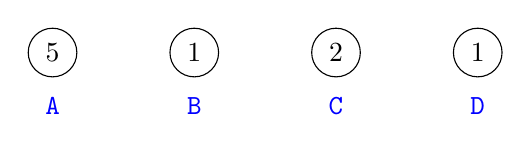
\begin{tikzpicture}[scale=0.9]
\node[draw, circle] (1) at (0,0) {$5$};
\node[draw, circle] (2) at (2,0) {$1$};
\node[draw, circle] (3) at (4,0) {$2$};
\node[draw, circle] (4) at (6,0) {$1$};

\node[color=blue] at (0,-0.75) {\texttt{A}};
\node[color=blue] at (2,-0.75) {\texttt{B}};
\node[color=blue] at (4,-0.75) {\texttt{C}};
\node[color=blue] at (6,-0.75) {\texttt{D}};

%\path[draw,thick,-] (4) -- (5);
\end{tikzpicture}
\end{center}
گرهی که نویسه \texttt{A} را نشان می‌دهد دارای وزن ۵ است زیرا نویسه \texttt{A} ۵ بار در رشته آمده است.
سایر وزن‌ها نیز به همین ترتیب محاسبه شده‌اند.

مرحله نخست، ترکیب گره‌های متناظر با نویسه‌های \texttt{B} و \texttt{D} است که هر دو وزن ۱ دارند.
نتیجه به این صورت است:
\begin{center}
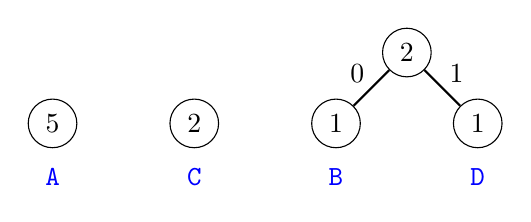
\begin{tikzpicture}[scale=0.9]
\node[draw, circle] (1) at (0,0) {$5$};
\node[draw, circle] (3) at (2,0) {$2$};
\node[draw, circle] (2) at (4,0) {$1$};
\node[draw, circle] (4) at (6,0) {$1$};
\node[draw, circle] (5) at (5,1) {$2$};

\node[color=blue] at (0,-0.75) {\texttt{A}};
\node[color=blue] at (2,-0.75) {\texttt{C}};
\node[color=blue] at (4,-0.75) {\texttt{B}};
\node[color=blue] at (6,-0.75) {\texttt{D}};

\node at (4.3,0.7) {0};
\node at (5.7,0.7) {1};

\path[draw,thick,-] (2) -- (5);
\path[draw,thick,-] (4) -- (5);
\end{tikzpicture}
\end{center}
پس از این، گره‌های با وزن ۲ ترکیب می‌شوند:
\begin{center}
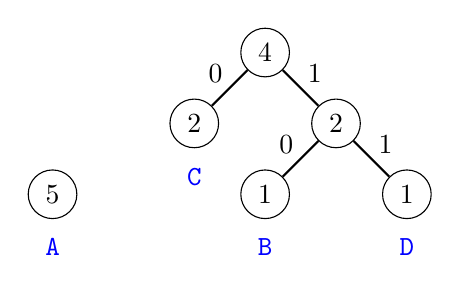
\begin{tikzpicture}[scale=0.9]
\node[draw, circle] (1) at (1,0) {$5$};
\node[draw, circle] (3) at (3,1) {$2$};
\node[draw, circle] (2) at (4,0) {$1$};
\node[draw, circle] (4) at (6,0) {$1$};
\node[draw, circle] (5) at (5,1) {$2$};
\node[draw, circle] (6) at (4,2) {$4$};

\node[color=blue] at (1,-0.75) {\texttt{A}};
\node[color=blue] at (3,1-0.75) {\texttt{C}};
\node[color=blue] at (4,-0.75) {\texttt{B}};
\node[color=blue] at (6,-0.75) {\texttt{D}};

\node at (4.3,0.7) {0};
\node at (5.7,0.7) {1};
\node at (3.3,1.7) {0};
\node at (4.7,1.7) {1};

\path[draw,thick,-] (2) -- (5);
\path[draw,thick,-] (4) -- (5);
\path[draw,thick,-] (3) -- (6);
\path[draw,thick,-] (5) -- (6);
\end{tikzpicture}
\end{center}
در نهایت، دو گره باقی‌مانده ترکیب می‌شوند:
\begin{center}
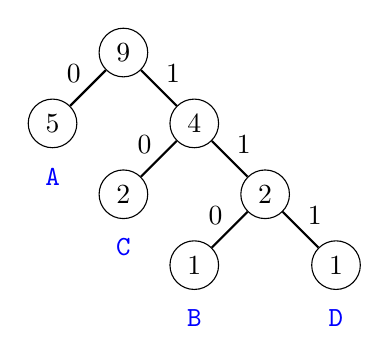
\begin{tikzpicture}[scale=0.9]
\node[draw, circle] (1) at (2,2) {$5$};
\node[draw, circle] (3) at (3,1) {$2$};
\node[draw, circle] (2) at (4,0) {$1$};
\node[draw, circle] (4) at (6,0) {$1$};
\node[draw, circle] (5) at (5,1) {$2$};
\node[draw, circle] (6) at (4,2) {$4$};
\node[draw, circle] (7) at (3,3) {$9$};

\node[color=blue] at (2,2-0.75) {\texttt{A}};
\node[color=blue] at (3,1-0.75) {\texttt{C}};
\node[color=blue] at (4,-0.75) {\texttt{B}};
\node[color=blue] at (6,-0.75) {\texttt{D}};

\node at (4.3,0.7) {0};
\node at (5.7,0.7) {1};
\node at (3.3,1.7) {0};
\node at (4.7,1.7) {1};
\node at (2.3,2.7) {0};
\node at (3.7,2.7) {1};

\path[draw,thick,-] (2) -- (5);
\path[draw,thick,-] (4) -- (5);
\path[draw,thick,-] (3) -- (6);
\path[draw,thick,-] (5) -- (6);
\path[draw,thick,-] (1) -- (7);
\path[draw,thick,-] (6) -- (7);
\end{tikzpicture}
\end{center}

اکنون همه گره‌ها در درخت هستند، بنابراین کد آماده است.
کلمه‌کدهای زیر از درخت قابل خواندن هستند:
\begin{center}
\begin{tabular}{rr}
نویسه & کلمه‌کد \\
\hline
\texttt{A} & 0 \\
\texttt{B} & 110 \\
\texttt{C} & 10 \\
\texttt{D} & 111 \\
\end{tabular}
\end{center}